\subsubsection{\stid{3.12} Sub-project: hypre}

\paragraph{Overview}
The {\sl hypre} software library \cite{hypre:homepage,hypre_design_impl_2006} provides high performance preconditioners and solvers for the solution of large sparse linear systems on massively parallel computers, with particular focus on algebraic multigrid solvers. One of {\sl hypre}’s unique features is the provision of a (semi)-structured interface, in addition to a traditional linear-algebra based interface. The semi-structured interface is appropriate for applications whose grids are mostly structured, but with some unstructured features. Examples include block-structured grids, composite grids in structured adaptive mesh refinement (AMR) applications, and overset grids. These interfaces give application users a more natural means for describing their linear systems, and provide access to methods such as structured multigrid solvers, which can take advantage of the additional information beyond just the matrix. Since current architecture trends are favoring regular compute patterns to achieve high performance, the ability to express structure has become much more important. The {\sl hypre} library provides both unstructured and structured multigrid solvers, which have shown excellent scalability on a variety of high performance computers, e.g Blue Gene systems (unstructured solver BoomerAMG has scaled up to 1.25 million MPI cores with a total of 4.5 million hardware threads). It is used by many ECP application teams, including ExaAM, Subsurface, ExaWind, CEED, and more. It requires a C compiler and an MPI implementation, but it also runs in an OpenMP environment. It also has GPU capabilities.

\paragraph{Key  Challenges}

While {\sl hypre}'s solvers contain much parallelism, their main focus is the solution of sparse linear systems, leading to  very large demands on memory bandwidth. In addition, the use of multiple levels, while greatly aiding convergence of the solvers, leads to decreasing systems sizes, number of operations and parallel efficiencies on coarser levels. Particularly the unstructured algebraic multigrid solver BoomerAMG\cite{HeYa2002}, which is {\sl hypre}'s most often used preconditioner, suffers from increasing communication complexities on coarser levels. Coarse grid operators are generated by multiplying three matrices leading to increasing numbers of nonzeroes per row in the resulting matrices and with it increasing numbers of neighbor processes. While BoomerAMG's solve phase mainly consists of matrix vector products and smoothing operations, which are fairly straight forward to parallelize, even on a GPU, its setup phase is highly complex, including many branches, a lot of integer operations as well as some sequential passages. Current  interpolation strategies that lead to best convergence and performance on distributed memory machines are not suitable for implementation on GPUs or similar architectures requiring extreme parallelism. Since {\sl hypre} is a mature product with many solvers and interdependent features, any significant changes that affect the whole library, are tedious and require much testing to ensure that the library stays backward compatible and no features are broken.

\paragraph{Solution Strategy}

Since computer architectures continue to change rapidly, it was important to come up with strategies that will facilitate future porting of the software. Therefore we developed and implemented a new memory model that addresses the use of different memory locations.
Since the upcoming computer architectures are heterogeneous with accelerators, we focus on enabling {\sl hypre} for GPUs. We have looked into various options, such as the use of CUDA, OpenMP 4.5, as well as RAJA and Kokkos. We limited the latter three options to the structured interface and solvers which are more natural candidates for such an approach due to their use of macros, called BoxLoops, for loops. We adopted a modular approach for the unstructured interface, which relies on the restructuring the solver components to use smaller kernels that are and/or will be implemented in CUDA for Nvidia GPUs. We will investigate the use of vendor conversion tools from CUDA to HIP and SYCL to port the unstructured solvers to upcoming exascale computers.

\paragraph{Recent Progress}

Previously, we enabled the structured solvers, SMG and PFMG\cite{AsFa1996}, both setup and solve phase, to completely run on GPUs, using both CUDA or OpenMP4.5, or use optional RAJA and Kokkos.
For our unstructured AMG solver BoomerAMG, we had implemented suitable CUDA kernels for setup and solve phase, which allowed AMG to run on GPUs for specific settings, but did not include our best interpolation operators. Recently, we added CUDA capabilities to create and assemble IJ matrices and vectors. Since our best interpolation operators are not suitable for GPU implementation, we designed a new class of interpolation operators based on sparse matrix operations\cite{LiSY2020} and implemented it on GPUs. We also ported aggressive coarsening to the GPU, which leads to decreased memory complexities and can also reduce overall run times. This included the implementation of a second strength matrix, required to get even coarser grids, and several two-stage interpolation operators also based on matrix-matrix operations and capable to deal with grid points that are further apart. Figure \ref{fig:27pt} and Figure \ref{fig:syslap} show two weak scaling studies comparing GPU and CPU implementations of AMG-PCG on Lassen, using 4 MPI tasks per node with 1 GPU per MPI task for the GPU version and 10 OpenMP threads per MPI task for the CPU version.

\begin{figure}[bth]
\centering
	\includegraphics[width=3.9in]{projects/2.3.3-MathLibs/2.3.3.12-SUNDIALS-hypre/mm-exti-27pt-200.png}
	%\includegraphics[width=3in]{mm-exti-27pt-200.png}
	\caption{\label{fig:27pt} Weak scaling study for AMG-PCG applied to a 3D 27pt diffusion problem on Lassen with 8M grid points per node comparing total run times (setup and solve) on GPUs with the new mm-ext+i interpolation (GPU), and on CPUs using ext+i interpolation (CPU), and adding aggressive coarsening with multipass interpolation on the first level (opt-CPU)}
\end{figure}

\begin{figure}[bth]
\centering
	\includegraphics[width=2.5in]{projects/2.3.3-MathLibs/2.3.3.12-SUNDIALS-hypre/a1-sysLap.png}
	%\includegraphics[width=3in]{a1-sysLap.png}
	\caption{\label{fig:syslap} Weak scaling study for AMG-PCG applied to a system of coupled Poisson problems with 3 variables per grid point on Lassen with 8M grid points (24M dofs) per node comparing CPU (dashed) and GPU (solid) total run times with (red) and without (blue) aggressive coarsening on the first level. Here CPU and GPU runs use mm-ext+e interpolation and two-stage mm-ext+e interpolation when using aggressive coarsening.}
\end{figure}

\paragraph{Next Steps}

We will pursue the following tasks:

\begin{itemize}
\item We will continue to add new GPU capabilities to {\sl hypre} and improve the performance of current capabilities. We will thoroughly investigate the performance on Nvidia GPUs and begin porting to AMD GPUs.
\item We also investigate and improve the performance of other unstructured solvers in {\sl hypre}, such as AMS and ILU and port components to GPUs where needed.
\end{itemize}
In addition, we will work with ECP application teams who are using {\sl hypre}, such as ExaWind, or would like to use it, to achieve best performance by tuning the solvers for them and potentially implementing suitable algorithmic changes.
